%%%%%%%% ICML 2023 EXAMPLE LATEX SUBMISSION FILE %%%%%%%%%%%%%%%%%

\documentclass{article}

% Recommended, but optional, packages for figures and better typesetting:
\usepackage{microtype}
\usepackage{graphicx}
\usepackage{subfigure}
\usepackage{booktabs} % for professional tables
\usepackage{svg}

\usepackage{tikz}
% Corporate Design of the University of Tübingen
% Primary Colors
\definecolor{TUred}{RGB}{165,30,55}
\definecolor{TUgold}{RGB}{180,160,105}
\definecolor{TUdark}{RGB}{50,65,75}
\definecolor{TUgray}{RGB}{175,179,183}

% Secondary Colors
\definecolor{TUdarkblue}{RGB}{65,90,140}
\definecolor{TUblue}{RGB}{0,105,170}
\definecolor{TUlightblue}{RGB}{80,170,200}
\definecolor{TUlightgreen}{RGB}{130,185,160}
\definecolor{TUgreen}{RGB}{125,165,75}
\definecolor{TUdarkgreen}{RGB}{50,110,30}
\definecolor{TUocre}{RGB}{200,80,60}
\definecolor{TUviolet}{RGB}{175,110,150}
\definecolor{TUmauve}{RGB}{180,160,150}
\definecolor{TUbeige}{RGB}{215,180,105}
\definecolor{TUorange}{RGB}{210,150,0}
\definecolor{TUbrown}{RGB}{145,105,70}

% hyperref makes hyperlinks in the resulting PDF.
% If your build breaks (sometimes temporarily if a hyperlink spans a page)
% please comment out the following usepackage line and replace
% \usepackage{icml2023} with \usepackage[nohyperref]{icml2023} above.
\usepackage{hyperref}


% Attempt to make hyperref and algorithmic work together better:
\newcommand{\theHalgorithm}{\arabic{algorithm}}

\usepackage[accepted]{icml2023}

% For theorems and such
\usepackage{amsmath}
\usepackage{amssymb}
\usepackage{mathtools}
\usepackage{amsthm}

% if you use cleveref..
\usepackage[capitalize,noabbrev]{cleveref}

%%%%%%%%%%%%%%%%%%%%%%%%%%%%%%%%
% THEOREMS
%%%%%%%%%%%%%%%%%%%%%%%%%%%%%%%%
\theoremstyle{plain}
\newtheorem{theorem}{Theorem}[section]
\newtheorem{proposition}[theorem]{Proposition}
\newtheorem{lemma}[theorem]{Lemma}
\newtheorem{corollary}[theorem]{Corollary}
\theoremstyle{definition}
\newtheorem{definition}[theorem]{Definition}
\newtheorem{assumption}[theorem]{Assumption}
\theoremstyle{remark}
\newtheorem{remark}[theorem]{Remark}

% Todonotes is useful during development; simply uncomment the next line
%    and comment out the line below the next line to turn off comments
%\usepackage[disable,textsize=tiny]{todonotes}
\usepackage[textsize=tiny]{todonotes}


% The \icmltitle you define below is probably too long as a header.
% Therefore, a short form for the running title is supplied here:
\icmltitlerunning{Project Report Template for Data Literacy 2023/24}

\begin{document}

\twocolumn[
\icmltitle{Satellite Density Evaluation: Investigating Satellite Presence above Tübingen}

% It is OKAY to include author information, even for blind
% submissions: the style file will automatically remove it for you
% unless you've provided the [accepted] option to the icml2023
% package.

% List of affiliations: The first argument should be a (short)
% identifier you will use later to specify author affiliations
% Academic affiliations should list Department, University, City, Region, Country
% Industry affiliations should list Company, City, Region, Country

% You can specify symbols, otherwise they are numbered in order.
% Ideally, you should not use this facility. Affiliations will be numbered
% in order of appearance and this is the preferred way.
\icmlsetsymbol{equal}{*}

\begin{icmlauthorlist}
\icmlauthor{Timo Lübbing}{equal,third}
\icmlauthor{Meike Oschmann}{equal,second}
\icmlauthor{Sebastian Volz}{equal,first}

\end{icmlauthorlist}

\icmlaffiliation{first}{ 5457430, sebastian.volz@student.uni-tuebingen.de, MSc Computer Science}
\icmlaffiliation{second}{ 6042587, meike.oschmann@student.uni-tuebingen.de, MSc Cognitive Science}
\icmlaffiliation{third}{ 5443129, timo.luebbing@student.uni-tuebingen.de, MSc Machine Learning}

% You may provide any keywords that you
% find helpful for describing your paper; these are used to populate
% the "keywords" metadata in the PDF but will not be shown in the document
\icmlkeywords{Machine Learning, ICML}

\vskip 0.3in
]

% this must go after the closing bracket ] following \twocolumn[ ...

% This command actually creates the footnote in the first column
% listing the affiliations and the copyright notice.
% The command takes one argument, which is text to display at the start of the footnote.
% The \icmlEqualContribution command is standard text for equal contribution.
% Remove it (just {}) if you do not need this facility.

%\printAffiliationsAndNotice{}  % leave blank if no need to mention equal contribution
\printAffiliationsAndNotice{\icmlEqualContribution} % otherwise use the standard text.

\begin{abstract}
In recent years, the Earth's orbital satellite population has substantially grown, primarily attributed to SpaceX's Starlink initiative. Concerns about the re-entry of satellites and space debris have been widely covered by media outlets. Our investigation assesses the likelihood to encounter falling satellites in the vicinity of Tübingen.
We leverage a publicly accessible API to retrieve real-time satellite locations. Using a kernel density estimate, we construct a \textit{danger heat map} illustrating satellite presence around Tübingen.
The density estimate reveals an elevated concentration of satellites along latitudes above $50^\circ$ N, forming a distinctive belt. This phenomenon corresponds with the Starlink satellite mesh. The operational border of Starlink orbits aligns with the observed high-density belt across all captures. Overall, our findings indicate that Tübingen is not situated in the identified high-density regions.
\end{abstract}

\section{Introduction}\label{sec:intro}
We are living under a sky full of stars - and full of more and more satellites. The first satellite, Sputnik-1, launched in 1957, marked the beginning of space exploration. Since then, thousands have been launched, serving various purposes such as communication, weather forecasting and navigation, contributing to our understanding of Earth and the galaxy. While in 2021, the number of satellites orbiting the earth has already increased to 4,877, it mounted to 7,560 in 2023 \cite{ucs_database}. 
SpaceX, a private aerospace company, initiated satellite deployment in 2019, with plans to launch a total of 12,000 satellites to provide global internet access.\\ 
In response to the increasing number of space objects, multiple media outlets have reported on the risk of reentering satellites. While in 2021 there was a $7\%$ chance of at least one person on the ground being seriously injure or killed by falling space debris, the risk is expected to increase to $61\%$ in 2035 \cite{FAA_report}. 
Consequently, we asked ourselves how likely it is to get hit by falling satellites in Tübingen. To explore this question, we analyzed real-time satellite location data using a publicly accessible API, allowing us to gather satellites based on our coordinates.\\
We employ 2-dimensional kernel density estimation to characterize the satellite distribution above Tübingen, generating a probability density surface. Assuming a strongly simplified correlation between the likelihood of re-entry events and high-density regions, we propose this density surface as a \textit{danger heat map} in Tübingen's vicinity. We expect a non-uniform satellite distribution in the sky above us and aim to attribute high-density areas to specific satellite categories, particularly the expanding constellation of Starlink satellites, which is expected to influence the overall density estimate.\\
Throughout the data capture and preprocessing, we addressed challenges outlined in Section \ref{sec:methods}. We present the \textit{danger heat map} around Tübingen and Starlink specific influences (Section \ref{sec:results}). We conclude by discussing high-density areas that correlate to the Starlink mesh and provide a general intuition for the local satellite re-entry risk in Tübingen (Section \ref{sec:conclusion}).
The source code for this project is available on our \href{https://github.com/timoluebbing/Satellites}{GitHub repository}.
\section{Data and Methods}\label{sec:methods}

\subsection{Data Collection}
\begin{figure}[h]
    \begin{center}
        \includegraphics[width=.6\columnwidth]{fig/above.png}
        \caption{API call ``above" to capture all satellites above the reference coordinates in a cone with angle $\theta$.}
        \label{fig:above}
    \end{center}
\end{figure}

We obtained our data using the ``above" function of the \href{https://www.n2yo.com/api/}{n2yo} API. The n2yo platform sources its data from the United States Space Surveillance Network, managed by the US Air Force Space Command (AFSPC). The ``above" function returns all objects within a given search angle $\theta$ above an observer's location (Figure \ref{fig:above}). This data includes latitude, longitude, altitude, satellite name, and a unique satellite catalog number (NORAD).\\
Two separate datasets were created through a systematic data retrieval processes. Initially, requests were sent at 5-second intervals for a duration of 30 minutes. Subsequently, additional data points were collected at 30-minute intervals over a 24-hour period. The reference point chosen was the coordinates of the Brechtbau (48.5269° N, 9.0632° W) in Tübingen, with an angular inclination set at $\theta=90$ degrees.
\begin{figure}
    \begin{center}
        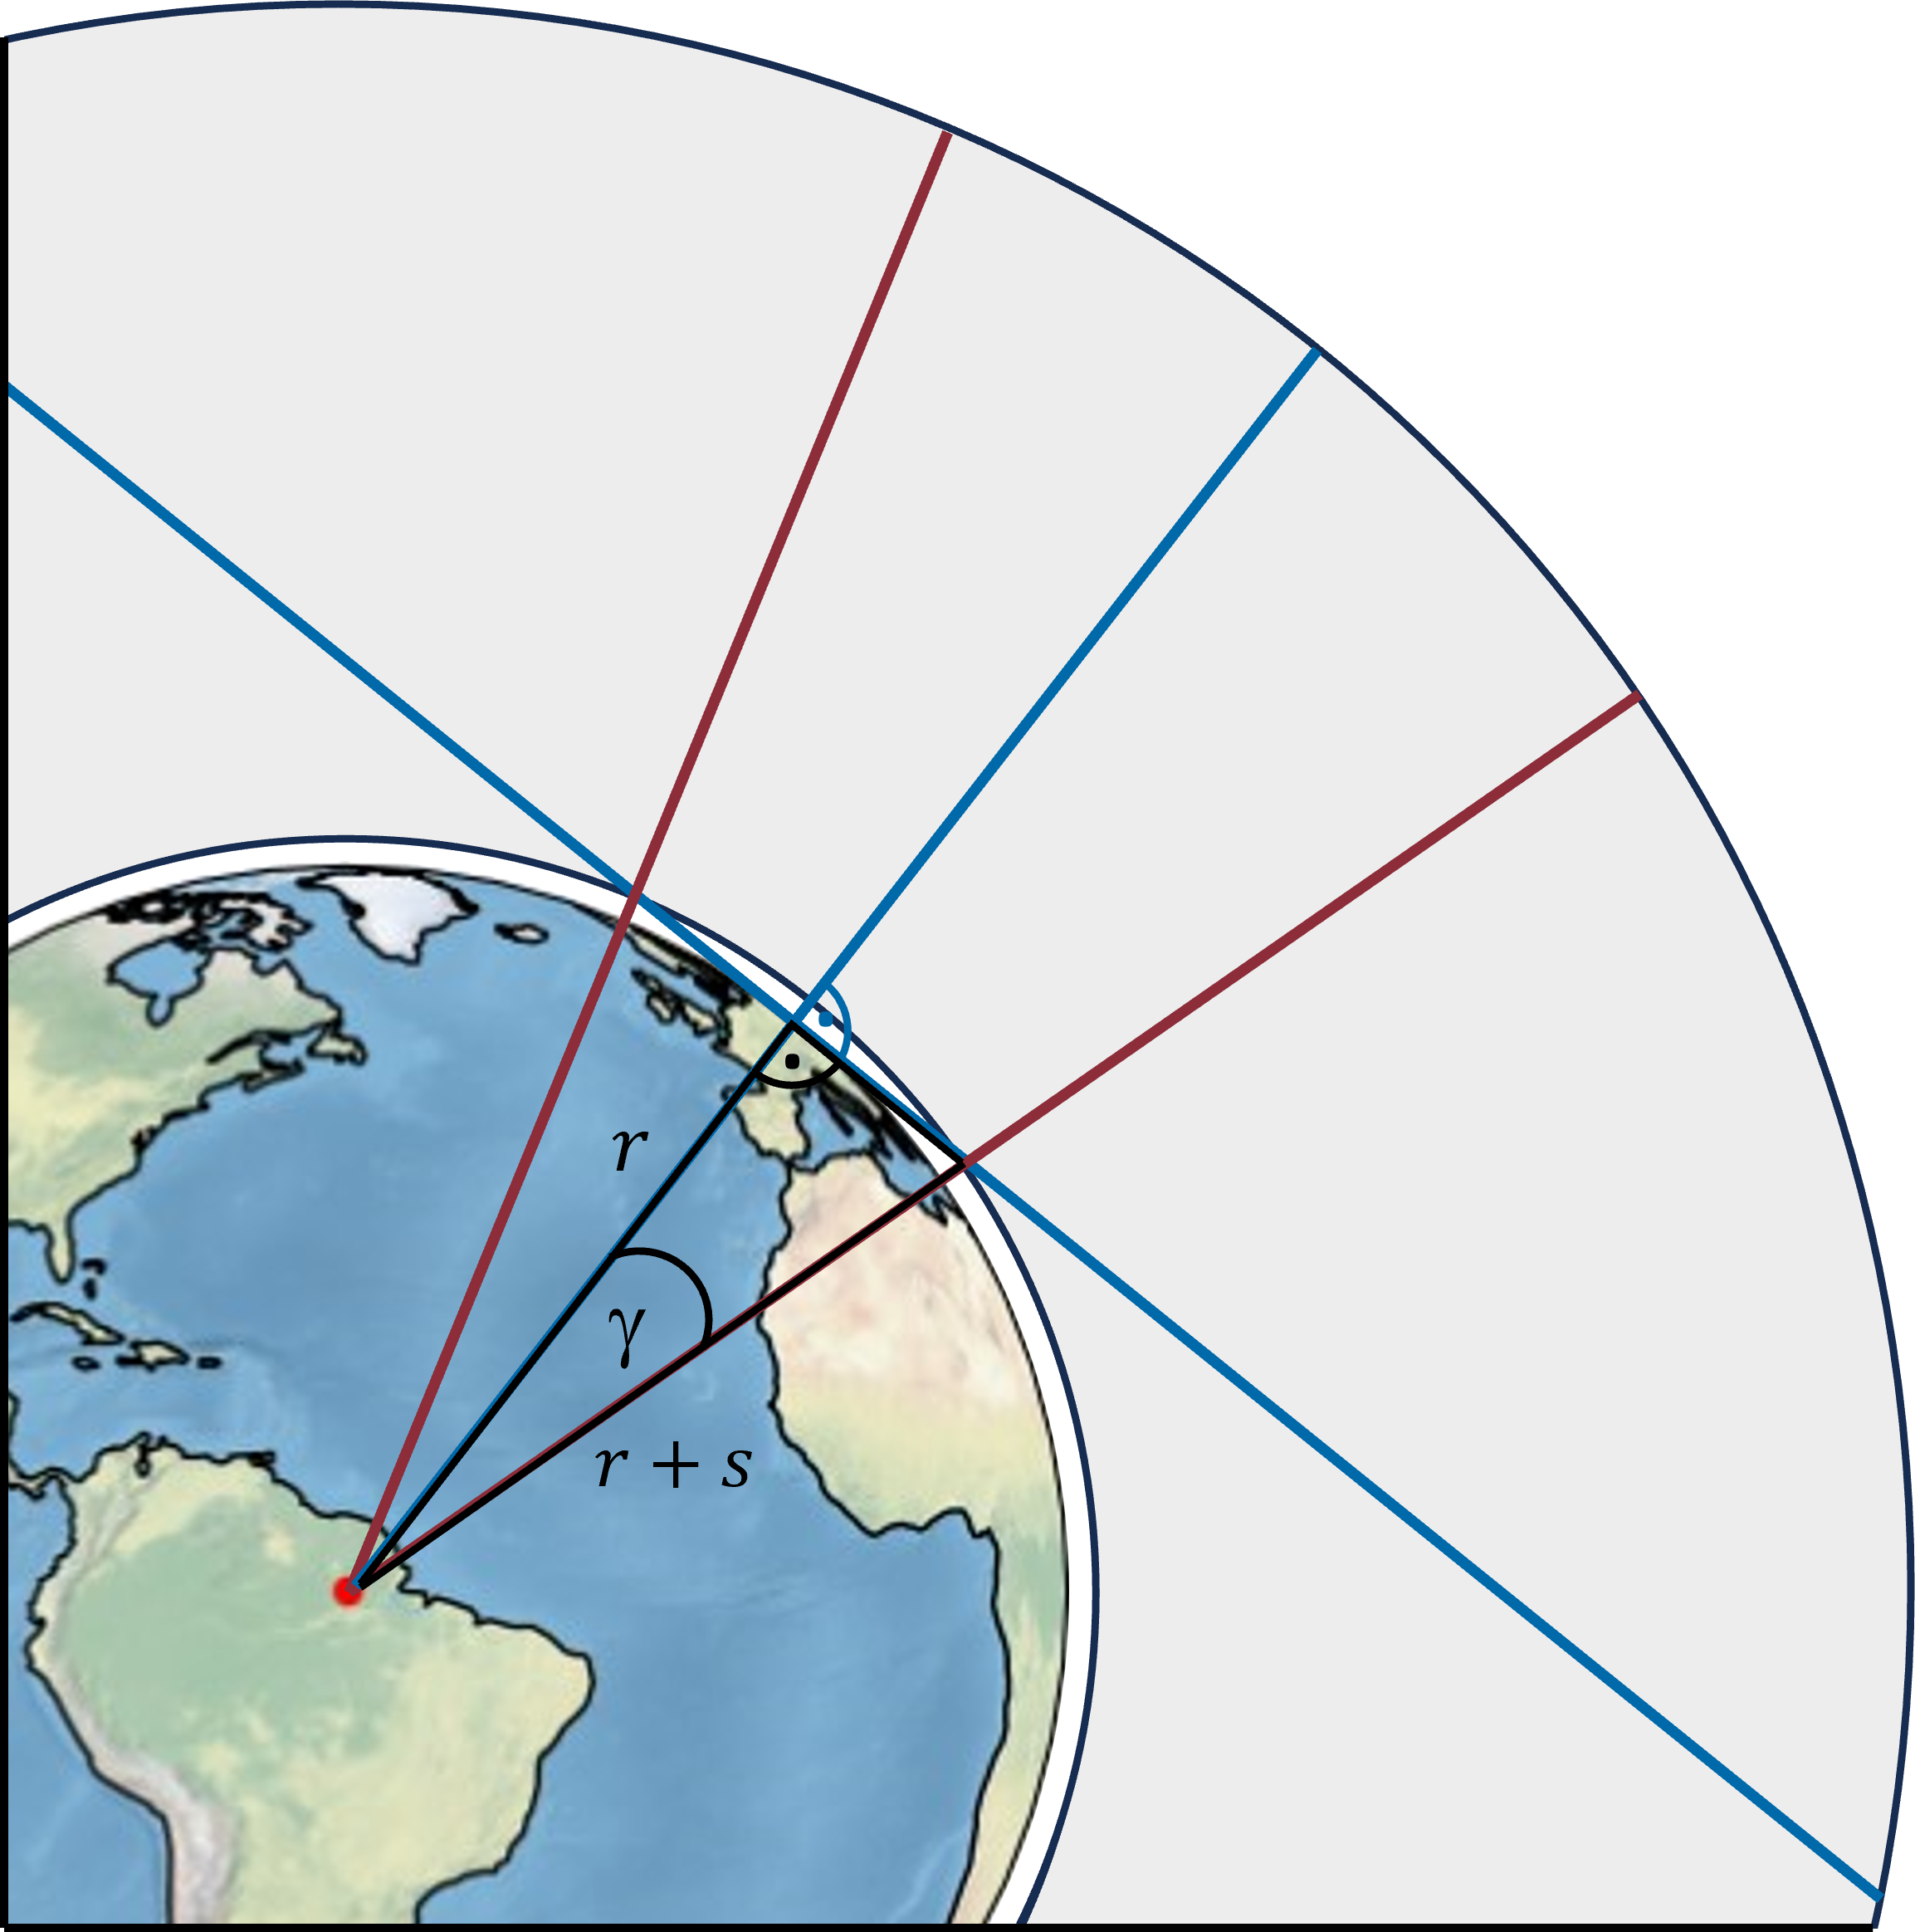
\includegraphics[width=.7\columnwidth]{fig/schema_final.png}
        \caption{Schematic plot of our satellite capture window. The blue line horizontal to the Earth's surface illustrates the search cone of 90° above Tübingen. Every satellite below this line is not captured by the API call. Between the red lines, the satellites of all altitudes are captured. This defines our localized capture area. With equation \ref{eq:gamma} and $r=6370$ km and $r+s=6370+200$ km, we calculate $\gamma$.}
        \label{fig:schematic_plot}
    \end{center}
\end{figure}
\begin{figure*}[h!]
    \begin{center}
        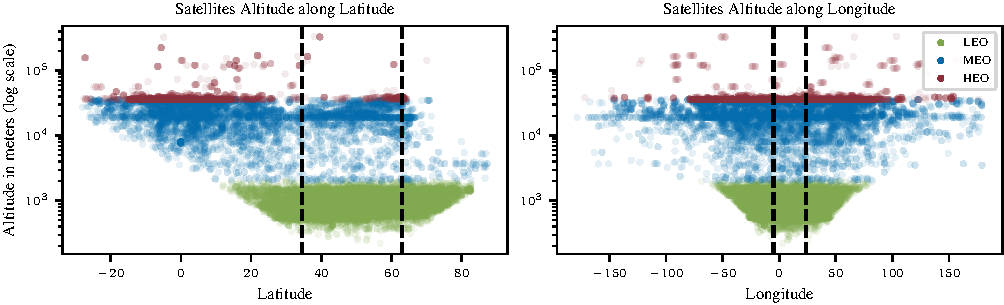
\includegraphics{fig/satellite_altitude.png}
        \caption{Satellite altitudes with respect to latitude \textit{(left)} and longitude \textit{(right)}. Satellites in Low Earth Orbit are visualized in green, Medium Earth Orbit satellites in blue, and High Earth Orbit satellites in red. The \textit{dashed lines} display our sample cutoff, defined as the spherical distance of $\gamma = 14.172^\circ$ centered around Tübingen. We continue to use this localized subset of satellites for our following analysis.}
        \label{fig:altitude}
    \end{center}
\end{figure*}

\subsection{Data Preprocessing}
We started by visualizing the raw data collected with a search angle of $\theta=45$ degrees and plotted the satellite distribution for 100 random time frames. 
We realized there was a hot-spot of satellites above Germany, together with a less dense distribution at the outside margin of the search window. 
To verify if this was due to a higher presence of satellites above middle Europe, we collected data above New Zealand. It followed a similar distribution, making us question the quality of our data. \\
Reinspecting the way the data was collected, we were able to resolve the problem. The search area was defined by a cone above the reference location. Towards the edge of the search cone, we would only capture satellites in high altitude (Figure \ref{fig:schematic_plot}).  
Exclusively in a small area around the reference point, the satellites in all altitudes were captured, explaining the observed hot-spot. Therefore, we increased the angle of the search cone to the maximum of $\theta=90$ degrees to capture a larger space around the reference location.\\\\ 
Aiming to extract the surface on the earth above which we capture all satellites, we geometrically calculate the angle $\gamma$ shown in Figure \ref{fig:schematic_plot}.
Therefore, we construct a triangle using the distance $r$ from the Earth's center to the reference point as the side adjacent to $\gamma$, and the line segment $r+s$ from the Earth's center to the intersection of the cone with the satellite belt as the hypotenuse. 
The angle, and thus the spherical distance, $\gamma$ is calculated with:
\begin{equation}{\label{eq:gamma}}
    \gamma = \arccos{\left( \frac{r}{r + s} \right)} =  14.1735^\circ
\end{equation}
where $r=6370$ km and $(r+s)=6370+200$ km.
Positions on the Earth are measured as latitude and longitude using the spherical geographic coordinate system. Since the unit of measurement is degree, we are able to extract a circle around the reference location using the angle $\gamma$ as the radius. 
The data is then filtered by the distance to the reference point in Tübingen. Points with a distance smaller or equal to $\gamma$ are kept.\\
The distance in spherical coordinates of two points $p=(r,\alpha,\beta)$ and $p'=(r',\alpha',\beta')$ with radius $r$, latitude $\alpha$ and longitude $\beta$ can be calculated according to the following equation:
\begin{multline}
      \mathbf{D} = \left(r^2+r'^2-2rr'(\sin{\alpha}\sin{\alpha'}\cos{(\beta-\beta')}\\
      + \cos{\alpha}\cos{\alpha'})\right)^{\frac{1}{2}}
\end{multline} 
Since in the Earth's coordinate system, the latitude takes the value $0^\circ$ at the equator instead of at the pole, latitude values need to be subtracted from $90^\circ$.\\\\
Having extracted the area around Tübingen above which all satellites are captured, we investigate the distribution of different types of satellites, most notably the distribution of Starlink satellites. 

\subsection{Data Analysis}
Filtering the satellites by their name allows us to compare the distribution of Starlink satellites to the distribution of the entire sample. 
To estimate the probability density function in a non-parametric way, kernel density estimation is used. The bandwidth of the Gaussian Kernel is calculated using Scott's Rule \cite{scott2015multivariate}:
\begin{equation}
   \setlength{\abovedisplayskip}{7pt}
   h = n^{-\frac{1}{(d+4)}}
   \setlength{\belowdisplayskip}{7pt}
\end{equation}
% $h = n^{-\frac{1}{(d+4)}}$
with $n$ the number of data points and $d$ the number of dimensions ($d = 2$, latitude and longitude in this case). We apply the gaussian\_kde function of the \textit{scipy.stats} library \cite{2020SciPy-NMeth}. To produce the heatmap in Figure \ref{fig:density}, the function is evaluated on a 2-dimensional grid spanning the visible cut-out of the map. Hence, Gaussian kernels were fit to each of the points on the grid and then summed up. 
% gaussian kernel, automatic bandwith selection, see here: https://docs.scipy.org/doc/scipy/reference/generated/scipy.stats.gaussian_kde.html#scipy.stats.gaussian_kde
% note that multimodal distributions tend to be oversmoothed :o
% univariate data?

\section{Results}\label{sec:results}
\begin{figure}[h]
    \begin{center}
        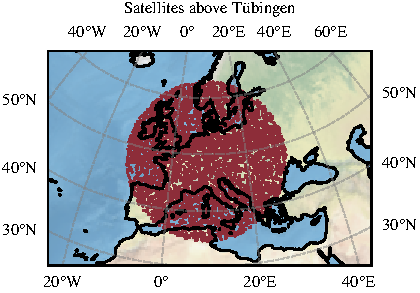
\includegraphics{fig/satellite_above_tuebingen.pdf}
        \caption{Localized satellites subset around Tübingen. We include all satellites where the distance to Tübingen is smaller than our spherical cutoff distance of $\gamma = 14.172^\circ$. Tübingen center coordinates are $48.782536^\circ$ N and $9.176995^\circ$ E. The kernel density estimations are performed on this localized subset.}
        \label{fig:tue-sample}
    \end{center}
\end{figure}
\subsection{Orbits at different altitudes}
We discover that at the edge of the search cone there are  only satellites in high altitude. 
Figure \ref{fig:altitude} shows the satellites of different orbits.
The low Earth orbit (LEO) covers the area of space below an altitude of 2,000 km. The High Earth orbit (HEO) comprises altitudes higher than 35,786 km, in-between the two is the middle Earth orbit (MEO). 
A special case is the geostationary orbit (GEO), which is at exactly 35,786 km altitude and is located in the Earth's equatorial plane. 
At this altitude, the GEO's orbital period matches the Earth's rotation, such that over the course of a day, to observers on the Earth, its satellites remain at the same position in the sky.
The plot reveals that the prominent belt of satellites we observe above the equator are the geostationary satellites. As visible in Figure \ref{fig:schematic_plot}, a search cone of 90° captured satellites above the equator in high altitude.\\

\subsection{Density Estimation}
The estimated density of both the entire captured sample and the Starlink satellites is shown in Figure \ref{fig:density}. Both display highest density at latitudes ranging from $50^\circ$ to $54^\circ$ N, creating a noticeable belt of higher satellite concentration. Additionally, there's a second area between $40^\circ$ and $44^\circ$ N that exhibits a relatively high density, though not as pronounced as the primary belt. This area is identified in both density estimates. The center reference point, Tübingen, is located between the two high-density belts. 
\begin{figure}[h]
    \begin{center}
        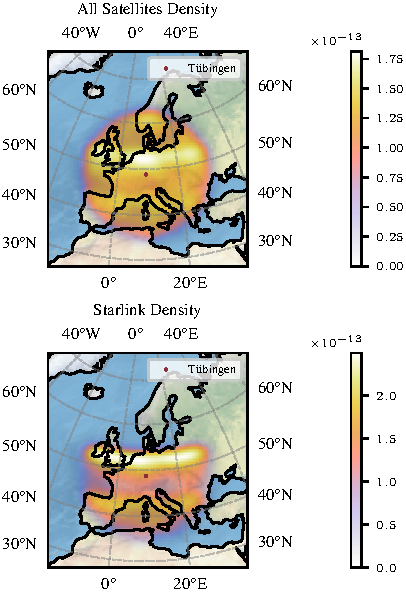
\includegraphics{fig/density_comparison.pdf}
        \caption{\textit{Danger head map}: We compare an estimate of the satellite density above Tübingen by category. The red marker indicates the location of Tübingen. The first figure \textit{(top)} shows the kernel density estimate for all captured satellites, and the second figure \textit{(bottom)} shows the equivalent for Starlink satellites only.  It is prominent that the band of increased likelihood in \textit{(top)} above $50^\circ$ N could be explained by the density of Starlink satellites.}
        \label{fig:density}
    \end{center}
\end{figure}

\subsection{Starlink Mesh}
Figure \ref{fig:mesh} illustrates the Starlink mesh, tracking a subset of distinct Starlink satellites (first digit of satellite ID is 1) over a 30-minute duration. Within this subset, all satellite orbits tangent a prominent operational boundary above $50^\circ$ N. In general, not all Starlink satellites follow this behavior. An animation of the entire set of Starlink satellites crossing Tübingen can be viewed in the README.md of our \href{https://github.com/timoluebbing/Satellites}{GitHub repository}.
\begin{figure}[h]
    \begin{center}
        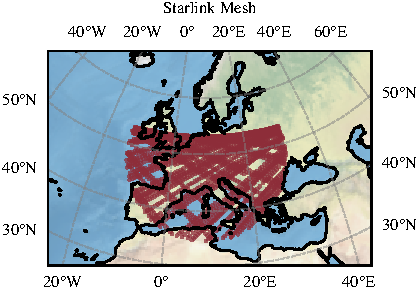
\includegraphics{fig/starlink_mesh.pdf}
        \caption{This figure shows a subset of Starlink satellites to illustrate the mesh of the Starlink satellite network. It contains 69 unique Starlink satellites across 64 time steps within 5 second data capture intervals. The boundary, at which the Starlink network of satellites is less likely to operate, is clearly visible in the figure.}
        \label{fig:mesh}
    \end{center}
\end{figure}

\section{Discussion \& Conclusion}\label{sec:conclusion}
After resolving data capture challenges, such as addressing the angle of the cone in which satellites were captured and accounting for spherical distances on the globe, we successfully refined our focus to a localized subset of satellites around Tübingen (Figure \ref{fig:tue-sample}). This subset includes the entire range of orbital altitudes (Figure \ref{fig:altitude}). 

As a result, we developed expressive satellite density estimates, yielding \textit{danger heat maps} for both our complete data capture and specifically for Starlink satellites. The densities, as illustrated in Figure \ref{fig:density}, indicate a non-uniform distribution of satellites across the sky.\\
Additionally, the consistent presence of high-density areas in both density estimates highlights the substantial influence of Starlink satellites on the overall satellite density.
Both uncover an elevated concentration of satellites along latitudes above $50^\circ$, forming a distinctive belt of high density. This observation aligns with the Starlink satellite mesh that is clearly visible in Figure \ref{fig:mesh}. \\
Regarding the imminent risk of satellite re-entry in Tübingen, the density figures lead us to the conclusion that Tübingen is notable for its comparatively low satellite density. This observation suggests a reduced likelihood of satellite re-entry events in the region. However, complex physical processes and non-linear descent paths of satellites preclude immediate conclusions regarding the potential impact of a satellite above Tübingen.

Subsequent research efforts could include the investigation of the second high-density belt above $40^\circ$ N, which is evident in both the overall density of captured satellites and the subset of Starlink satellites. Finally, we aim to calculate the probability and associated risk of encountering re-entering satellites in Tübingen. This should involve considering the temporal dimension and various statistical properties behind the physics of satellite re-entries.


\section*{Contribution Statement}
Sebastian Volz collected satellites data using API calls and was responsible for satellite animations. Meike Oschmann and Timo Lübbing performed the data preparation and analysis by means of kernel density estimation. Both contributed to producing visualizations. All authors jointly wrote the text of this report. In general, each team member contributed equally in work. 


\newpage

\bibliography{bibliography}
\bibliographystyle{icml2023}

\end{document}
